Internet Relay Chat (oder kurz IRC) bezeichnet ein vollkommen textbasiertes Chat-System. Hier treffen sich die Teilnehmer in sogenannten Channels und k�nnen in diesen Channels miteinander schreiben. Jeder Benutzer kann jederzeit einen neuen Channel erstellen. Au�erdem ist es m�glich sogenannte Querys zu erstellen, welche die Kommunikation zwischen nur zwei Gespr�chsteilnehmern erm�glicht.

\subsection{Geschichte}

Die erste Version eines solchen Chat-Netzwerks entstand 1985 im BITNET, einem Netzwerk von Gro�rechnern in den USA. Damals noch unter dem Namen Relay Chat. Zwei Studenten von der Universit�t Oulu, in Finnland �bertrugen dieses System 1988 auf das Internet. Die erste Version dieses Chat-Netzwerks erlangte schnell Beliebtheit, sodass bald weitere Unabh�ngige IRC Netze entstanden.

\subsection{Allgemein}

Ein IRC-Netzwerk besteht aus mehreren miteinander verbundenen Servern, welche auch Relay-Station genannt werden. Jeder Chat Teilnehmer verbindet sich immer mit einem Server und klingt sich somit in das Netz ein. Ein besonderes Merkmahl des IRC-Netzwerks ist, dass zwischen zwei Teilnehmern des Chats immer nur eine Verbindung besteht. Dies war historisch sehr bedeutsam, da fr�her die Leitungskapazit�t sehr begrenzt war. So wird jede Nachricht die von den Benutzern, die mit einem Server verbunden sind, nur �ber einen Kanal an einen weiteren Server und somit an deren Teilnehmer geschickt. Dieser Server schickt seine Nachricht daraufhin an den n�chsten Server weiter. Diese Funktionsweise sorgt f�r eine sehr geringe Menge an Datenverkehr, jedoch fehlt gleichzeitig jede Art von Redundanz. So kann es beim Ausfall eines Servers passieren, dass sich ein Netz in zwei kleinere Netze aufspaltet zwischen denen keine Verbindung mehr besteht.

\subsection{Technische Eigenschaften}

IRC ist ein auf IP und TCP basierendes Protokoll. Die gesamte Kommunikation besteht aus Textnachrichten mit einer maximalen L�nge von 512 Zeichen. Diese Textnachrichten enthalten einen Absender, einen Befehl und je nach Befehl eventuelle Befehlsparameter. Auf einen Befehl kann eine Antwort des Servers folgen, dies ist jedoch von Befehl zu Befehl und von Server zu Server unterschiedlich. Im Laufe der Zeit entwickelten sich au�erdem verschiedene Erweiterungen zum IRC Protokoll, welche unter anderem den Aufbau der Nachrichten �ndern. 

\subsection{Verschl�sselung}

Ob und wie Nachrichten verschl�sselt werden ist von Netz zu Netz unterschiedlich. In den meisten F�llen wird entweder gar nicht verschl�sselt oder eine �ber SSL/TLS verschl�sselte Verbindung benutzt. Verschiedene Erweiterungen benutzen hier ebenfalls verschiedene Verschl�sselungen.

\begin{figure}[h]
  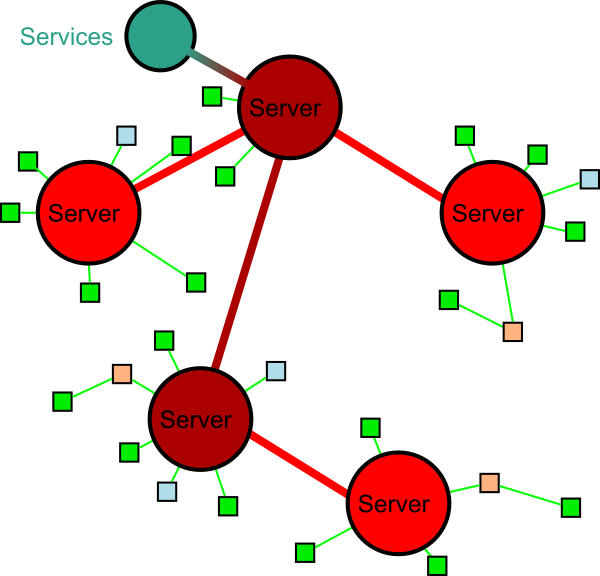
\includegraphics[width=\linewidth]{Ircnetz.png}
  \caption{Schematischer Aufbau eines IRC-Netzes.}
  \label{abb:Ircnetz}
\end{figure}

